% 第 17 题四棱锥 A-EFCB：按固定源内容流矢量层精确值复刻（1 pt → 0.03515 cm，与全库同制）。
% 原点取底左顶点 E（源页 (308.2850, 275.6570) pt），y 向上。
% 源实测：A 锥顶 (324.7547,173.4654)、B 底前、C 底右、F 底后被遮、O 为 EF 精确中点（差 <0.001 pt）。
% 实线 5 条（BE、EA、AB、BC、AC）；虚线 5 条（EF、OA 锥高严格竖直、OC、FA、FC）节距 2.9888/2.9888。
% 本图系示意图：EF 与 BC 图上仅近平行（差 0.18°）、非按题设比例（EF:BC 实测 1.549）；六标签无下标、无压线。
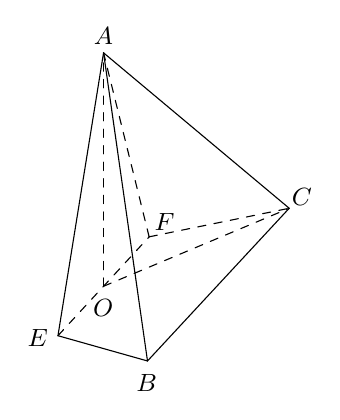
\begin{tikzpicture}[x=0.03515cm,y=0.03515cm,every node/.style={font=\small,inner sep=0pt},
  gl/.style={line width=0.3985bp,line cap=round,line join=round}]
% ===== 实线 5 条 =====
\draw[gl] (32.3442,-9.1279)--(0,0);            % B→E
\draw[gl] (0,0)--(16.4697,102.1916);           % E→A
\draw[gl] (16.4697,102.1916)--(32.3442,-9.1279); % A→B
\draw[gl] (32.3442,-9.1279)--(83.5393,46.0360);  % B→C
\draw[gl] (16.4697,102.1916)--(83.5393,46.0360); % A→C
% ===== 虚线 5 条（被遮棱与辅助线）=====
\draw[gl,dash pattern=on 2.9888pt off 2.9888pt] (0,0)--(32.9395,35.7175);                 % E→F
\draw[gl,dash pattern=on 2.9888pt off 2.9888pt] (16.4697,17.8586)--(16.4697,102.1916);     % O→A 锥高
\draw[gl,dash pattern=on 2.9888pt off 2.9888pt] (16.4697,17.8586)--(83.5393,46.0360);      % O→C
\draw[gl,dash pattern=on 2.9888pt off 2.9888pt] (32.9395,35.7175)--(16.4697,102.1916);     % F→A
\draw[gl,dash pattern=on 2.9888pt off 2.9888pt] (32.9395,35.7175)--(83.5393,46.0360);      % F→C
% ===== 六顶点标签（照源字形包围盒中心定位）=====
\node at (16.4700,108.2020) {\(A\)};
\node at (-7.2800,-0.9630) {\(E\)};
\node at (32.0800,-17.0630) {\(B\)};
\node at (88.0950,50.0070) {\(C\)};
\node at (38.5500,41.0970) {\(F\)};
\node at (16.3200,9.9220) {\(O\)};
\end{tikzpicture}
